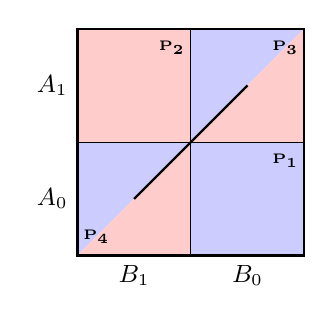
\begin{tikzpicture}[scale=1.2]
    % P2: A_H B_H (top-left)
    \draw[fill=red!20] (-1.8, 0.6) rectangle (-0.6, 1.8);
    \node[font=\tiny, black] at (-0.8, 1.6) {$\mathbf{P_2}$};
    
    % P3: A_H B_L (top-right) - diagonal split with P4 using P1 and P2 colors
    \fill[blue!20] (-0.6, 0.6) -- (-0.6, 1.8) -- (0.6, 1.8) -- cycle;
    \fill[red!20] (-0.6, 0.6) -- (0.6, 0.6) -- (0.6, 1.8) -- cycle;
    \draw (-0.6, 0.6) rectangle (0.6, 1.8);
    \node[font=\tiny, black] at (0.4, 1.6) {$\mathbf{P_3}$};
    
    % P4: A_L B_H (bottom-left) - diagonal split with P3 using P1 and P2 colors
    \fill[blue!20] (-1.8, -0.6) -- (-1.8, 0.6) -- (-0.6, 0.6) -- cycle;
    \fill[red!20] (-1.8, -0.6) -- (-0.6, -0.6) -- (-0.6, 0.6) -- cycle;
    \draw (-1.8, -0.6) rectangle (-0.6, 0.6);
    \node[font=\tiny, black] at (-1.6, -0.4) {$\mathbf{P_4}$};
    
    % P1: A_L B_L (bottom-right)
    \draw[fill=blue!20] (-0.6, -0.6) rectangle (0.6, 0.6);
    \node[font=\tiny, black] at (0.4, 0.4) {$\mathbf{P_1}$};
    
    % Line connecting P3 and P4 centers
    \draw[black, thick] (-1.2, 0) -- (0, 1.2);
    
    % Outer border
    \draw[thick] (-1.8, -0.6) rectangle (0.6, 1.8);
    
    % Labels for inputs
    % Vertical axis (A) - left side
    \node[left, font=\small] at (-1.8, 1.2) {$A_1$};
    \node[left, font=\small] at (-1.8, 0) {$A_0$};
    
    % Horizontal axis (B) - bottom
    \node[below, font=\small] at (-1.2, -0.6) {$B_1$};
    \node[below, font=\small] at (0, -0.6) {$B_0$};
\end{tikzpicture}
